%Autor: Simon Walker
%Version: 1.0
%Datum: 19.04.2020
%Lizenz: CC BY-NC-SA

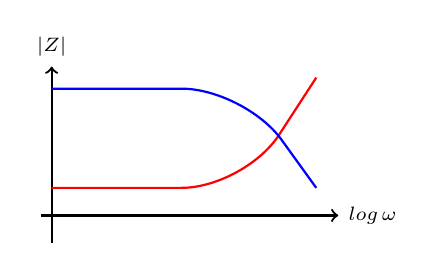
\begin{tikzpicture}[smooth, xscale=0.7, yscale=0.7]
	% Achsen
	\draw[->, thick] (-0.2,0) -- (5.2,0) node[right] {$\scriptstyle log \, \omega$}; % Horizontal
	\draw[->, thick] (0,-0.5) -- (0,2.7) node[above] {$ \scriptstyle \left|Z\right|$}; % Vertikal
	
	%Impedanzfunktion Serie (kleines R)
	\draw [red, thick, rounded corners=8mm] 
		(0, 0.5) -- (3.5, 0.5) -- (4.8, 2.5);
		
	%Impedanzfunktion Parallel (grosses R)
	\draw [blue, thick, rounded corners=8mm] 
	(0, 2.3) -- (3.5, 2.3) -- (4.8, 0.5);
	
\end{tikzpicture}
